%=========================================================
\chapter{Simulation-Based Swaption Pricing and Calibration}
\label{chap:pricing_methodology}
%=========================================================

The previous chapter examined whether the trained encoder--decoder model can be used as a stable forward scenario generator. We now ask whether the same model can be used for swaption pricing. This is a stronger requirement than curve reconstruction: pricing depends not only on the current decoded curve, but also on the distribution of future swap rates, discount factors and annuities under the risk-neutral measure.

The chapter develops this question in three steps. We first define the Monte Carlo pricing pipeline used throughout. We then diagnose why the pretrained model fails to price correctly: simulated paths leave the decoder's reliable region, and the historical drift introduces a systematic forward bias that cannot be corrected by rescaling the diffusion alone. Finally, we present a structural fix rooted in Girsanov's theorem: a single \(4\times4\) market-price-of-risk matrix \(\Lambda\) is trained against observed swaption prices while all neural-network weights remain frozen, and the resulting risk-neutral drift corrects the forward bias with the level factor receiving the largest adjustment.

%=========================================================
\section{Monte Carlo Swaption Pricing}
\label{sec:swaption_pricing_methodology}
%=========================================================

We now specialise the simulation-based pricing framework to European swaptions. The objective is to compute the option payoff on each simulated path and then average the discounted payoffs to obtain a time-zero price.

The section first defines the underlying swap and the at-the-money strike. It then derives the pathwise swap rate and payoff at expiry, before introducing the Monte Carlo estimator and the Bachelier convention used to express prices as implied normal volatilities.

\subsection{Swaption payoff and pathwise swap rate}
\label{subsec:swaption_payoff}

A European swaption gives the holder the right, but not the obligation, to enter into an interest-rate swap at a future exercise date \(T_e\). The underlying swap starts at \(T_e\) and has length \(T_s=n\delta\), where \(n\in\mathbb N\) is the number of fixed-leg payment periods and \(\delta>0\) is the fixed-leg accrual period. In the implementation, we use annual accrual, so \(\delta=1\). The fixed-leg payment dates are therefore
\[
T_e+\delta,\; T_e+2\delta,\; \dots,\; T_e+n\delta.
\]

The fixed rate agreed in the swaption contract is called the strike and is denoted by \(K\). In general, a swaption can be specified with any strike. In this thesis, we focus on at-the-money swaptions, following the market quoting convention for normal swaption volatilities. A swaption is at the money when the strike is equal to the current forward swap rate of the underlying swap.

The forward swap rate is the par fixed rate, observed at time zero, for a swap starting at \(T_e\) and ending at \(T_e+n\delta\). Given the time-zero discount curve \(P(0,T)\), the corresponding swap annuity is
\[
\mathcal A_0
=
\delta \sum_{j=1}^{n} P(0,T_e+j\delta),
\]
and the forward swap rate is
\[
F_0
=
\frac{P(0,T_e)-P(0,T_e+n\delta)}{\mathcal A_0}.
\]
For an at-the-money swaption, the strike is therefore chosen as
\[
K = F_0.
\]
This choice makes the underlying forward-starting swap have zero value at inception, but the swaption itself still has positive value due to the optionality.

For each simulated path \(m=1,\dots,N_{\mathrm{MC}}\), the latent state is simulated forward to the option expiry \(T_e\). The decoder then produces a zero-coupon bond curve at expiry. Since the decoder is expressed in terms of time to maturity, the pathwise curve is written as
\[
\tau \mapsto P^{(m)}(T_e,\tau),
\]
where \(m\) indexes the Monte Carlo path and \(P^{(m)}(T_e,\tau)\) denotes the price at time \(T_e\), on path \(m\), of a zero-coupon bond maturing \(\tau\) years later.

At expiry, the underlying swap is spot-starting: it starts immediately at \(T_e\) and has payment dates \(T_e+\delta,\dots,T_e+n\delta\). In time-to-maturity notation, these payment dates correspond to maturities
\[
\delta,\;2\delta,\;\dots,\;n\delta
\]
measured from \(T_e\). The pathwise swap annuity at expiry is therefore
\[
\mathcal A^{(m)}(T_e)
=
\delta \sum_{j=1}^{n} P^{(m)}(T_e,j\delta),
\]
and the corresponding pathwise par swap rate is
\[
S^{(m)}(T_e)
=
\frac{1-P^{(m)}(T_e,n\delta)}
{\mathcal A^{(m)}(T_e)}.
\]
Here the numerator uses \(P^{(m)}(T_e,0)=1\), since the floating leg of a spot-starting swap has value \(1-P^{(m)}(T_e,n\delta)\) under the single-curve assumption.

Let \(\mathcal N>0\) denote the notional. A payer swaption gives the holder the right to enter a payer swap, meaning that the holder pays the fixed rate \(K\) and receives the floating rate. It is therefore valuable when the market swap rate at expiry exceeds the strike. The payer payoff on path \(m\) is
\[
X^{(m),\mathrm{pay}}_{T_e}
=
\mathcal N\,\mathcal A^{(m)}(T_e)
\max\bigl(S^{(m)}(T_e)-K,0\bigr).
\]
A receiver swaption gives the holder the right to enter a receiver swap, meaning that the holder receives the fixed rate \(K\) and pays the floating rate. It is therefore valuable when the market swap rate at expiry is below the strike. The receiver payoff is
\[
X^{(m),\mathrm{rec}}_{T_e}
=
\mathcal N\,\mathcal A^{(m)}(T_e)
\max\bigl(K-S^{(m)}(T_e),0\bigr).
\]

\subsection{Monte Carlo estimator}
\label{subsec:mc_estimator}

The payoff is discounted back to time \(0\) using the pathwise bank account discount factor computed during simulation. Denoting this factor on path \(m\) by
\[
D^{(m)}_{T_e}
=
\exp\left(-\int_0^{T_e} r_s^{(m)}\,ds\right),
\]
the discounted present value on path \(m\) is
\[
V_0^{(m)}
=
D^{(m)}_{T_e} X^{(m)}_{T_e},
\]
where \(X^{(m)}_{T_e}\) denotes either the payer or receiver payoff defined above. In the implementation, the integral in the discount factor is approximated on the simulation grid using the trapezoidal rule, consistent with the discount-factor discretisation described in Chapter~\ref{chap:simulation}.

The time-zero swaption price is then estimated by the Monte Carlo average
\[
\widehat V_0
=
\frac{1}{N_{\mathrm{MC}}}
\sum_{m=1}^{N_{\mathrm{MC}}} V_0^{(m)}.
\]

To assess numerical uncertainty, we also report the sample standard deviation of the discounted pathwise payoffs,
\[
\widehat{\mathrm{SD}}_{\mathrm{MC}}
=
\sqrt{
\frac{1}{N_{\mathrm{MC}}-1}
\sum_{m=1}^{N_{\mathrm{MC}}}
\left(V_0^{(m)}-\widehat V_0\right)^2
},
\]
and the associated Monte Carlo standard error
\[
\widehat{\mathrm{SE}}_{\mathrm{MC}}
=
\frac{\widehat{\mathrm{SD}}_{\mathrm{MC}}}{\sqrt{N_{\mathrm{MC}}}}.
\]

\subsection{Bachelier swaption formula and implied normal volatility}
\label{subsec:bachelier_formula}

To report swaption prices in market-standard volatility units, we use the Bachelier normal-volatility framework. The relevant numeraire for a forward swap rate is the swap annuity,
\[
\mathcal A(t)
=
\delta\sum_{j=1}^{n} P(t,T_e+j\delta).
\]
The probability measure associated with this numeraire is called the annuity measure and is denoted by \(\mathbb Q^{\mathcal A}\). Under this measure, the forward swap rate is a martingale. This is analogous to a single-period forward rate being a martingale under its corresponding forward measure, but with the swap annuity replacing the zero-coupon bond numeraire.

In the Bachelier normal model \citep{Bachelier1900}, the forward swap rate is modelled as an arithmetic Brownian motion under the annuity measure:
\begin{equation}
    dF(t) = \sigma_N\, dW^{\mathcal A}(t),
    \label{eq:bachelier_sde}
\end{equation}
where \(\sigma_N>0\) is the normal volatility. The term normal volatility refers to the volatility parameter in this arithmetic, normally distributed model for rate changes. It is quoted in absolute rate units, often basis points per square-root year. The model is convenient in low- and negative-rate environments because it allows the forward swap rate to take negative values.

Under~\eqref{eq:bachelier_sde}, the time-zero price of a payer swaption with notional \(\mathcal N\), strike \(K\), option expiry \(T_e\), forward swap rate \(F\), and swap annuity \(\mathcal A_0\) is
\begin{equation}
    V^{\mathrm{pay}}
    =
    \mathcal N \mathcal A_0
    \Bigl[
        (F-K)\Phi(d)
        +
        \sigma_N\sqrt{T_e}\,\phi(d)
    \Bigr],
    \qquad
    d =
    \frac{F-K}{\sigma_N\sqrt{T_e}},
    \label{eq:bachelier_payer}
\end{equation}
where \(\Phi\) and \(\phi\) denote the standard normal distribution function and density, respectively. For a receiver swaption, the corresponding price is
\begin{equation}
    V^{\mathrm{rec}}
    =
    \mathcal N \mathcal A_0
    \Bigl[
        (K-F)\Phi(-d)
        +
        \sigma_N\sqrt{T_e}\,\phi(d)
    \Bigr].
    \label{eq:bachelier_receiver}
\end{equation}

For a market at-the-money swaption, the strike is \(K=F_0\), where \(F_0\) is the market forward swap rate observed at time zero. Taking \(F=F_0\), we have \(d=0\), and the Bachelier price reduces to
\begin{equation}
    V^{\mathrm{ATM}}
    =
    \mathcal N \mathcal A_0
    \frac{\sigma_N\sqrt{T_e}}{\sqrt{2\pi}}.
    \label{eq:bachelier_atm}
\end{equation}
This formula is used to convert market ATM normal-volatility quotes into price targets:
\begin{equation}
    V^{(i)}_{\mathrm{mkt}}
    =
    \mathcal N \mathcal A^{(i)}_0
    \frac{\sigma^{(i)}_{\mathrm{mkt}}\sqrt{T_e^{(i)}}}{\sqrt{2\pi}}.
    \label{eq:pricing_target}
\end{equation}

Conversely, after Monte Carlo pricing, an at-the-money model price can be converted back into an implied normal volatility by
\begin{equation}
    \widehat{\sigma}_{N,\mathrm{mod}}^{\mathrm{ATM}}
    =
    \frac{\widehat V_{\mathrm{MC}}\sqrt{2\pi}}
    {\mathcal N \mathcal A_0\sqrt{T_e}}.
    \label{eq:implied_vol_atm}
\end{equation}
This is the reporting convention used throughout. The focus in this chapter is exclusively on at-the-money swaptions and the ATM volatility surface across the three-by-three expiry--tenor grid.

The Bachelier Delta of a payer swaption is
\[
\Delta
=
\frac{\partial V^{\mathrm{pay}}}{\partial F}
=
\mathcal N\mathcal A_0\Phi(d).
\]
At the money, \(d=0\), so
\[
\Delta^{\mathrm{ATM}}
=
\frac12\mathcal N\mathcal A_0.
\]
This identity is used later as a benchmark: in the Bachelier model, a correctly centred market at-the-money payer swaption has \(d=0\), so the annuity-measure exercise probability \(\Phi(d)\) is \(50\%\).


%=========================================================
\section{Pricing Diagnostics}
\label{sec:pricing_diagnostics_ch}
%=========================================================

Applying the Monte Carlo pricing pipeline to the pretrained stable model reveals two distinct barriers. We diagnose them in turn: first the decoder coverage problem arising from off-manifold latent paths, and then a structural forward bias arising from the difference between the historical drift and the risk-neutral drift. Together these two diagnostics motivate the Lambda market-price-of-risk fix in Section~\ref{sec:lyashenko}.

%----------------------------------------------------------
\subsection{Decoder Coverage and Latent Displacement}
\label{sec:can_pretrained_model_price}
%----------------------------------------------------------

The encoder--decoder model from Chapter~\ref{chap:encoderdecodermodel} was trained to minimise reconstruction error on observed swap curves. Swaption pricing places an additional requirement on the model. The pricing pipeline encodes the initial swap curve into a latent state, simulates the latent SDE forward to the option expiry, and then decodes the simulated latent states into zero-coupon bond curves. These simulated latent states need not coincide with the encoded historical states seen during reconstruction training.

\begin{description}[
    style=unboxed,
    leftmargin=0pt,
    labelindent=0pt,
    labelsep=0.5em
]

\item[The pricing pipeline as an off-manifold test.]
The Monte Carlo swaption pricing framework can be viewed as a test of the trained encoder--decoder model away from the pure reconstruction setting. Starting from an observed swap curve, the encoder produces an initial latent state \(z_0\). The latent SDE is then simulated forward to the option expiry, producing a terminal latent state \(z_{T_e}^{(m)}\) on each Monte Carlo path. Finally, the decoder maps \(z_{T_e}^{(m)}\) into a zero-coupon bond curve, from which the pathwise swap rate, annuity and payoff are computed.

For reconstruction, the decoder is only required to behave well at encoded historical states of the form \(z=E(S)\), where \(S\) is an observed swap curve. For pricing, however, it must also behave well at simulated latent states reached by the SDE. This is a stronger requirement. If the simulated states lie outside the region where the decoder has learned to produce valid discount curves, the resulting swaption prices can become unreliable even if the reconstruction error on observed curves is small.

We first examine decoder robustness in isolation, before considering the SDE dynamics. For an encoded point \(z_0\), we generate perturbed latent states
\[
z = z_0 + \varepsilon \eta,
\qquad
\eta \sim \mathcal N(0,I_\ell),
\]
and measure the fraction of decoded curves that are fully finite. This gives a simple diagnostic of how far the decoder can be moved away from encoded historical states before numerical failures occur.

\begin{figure}[H]
    \centering
    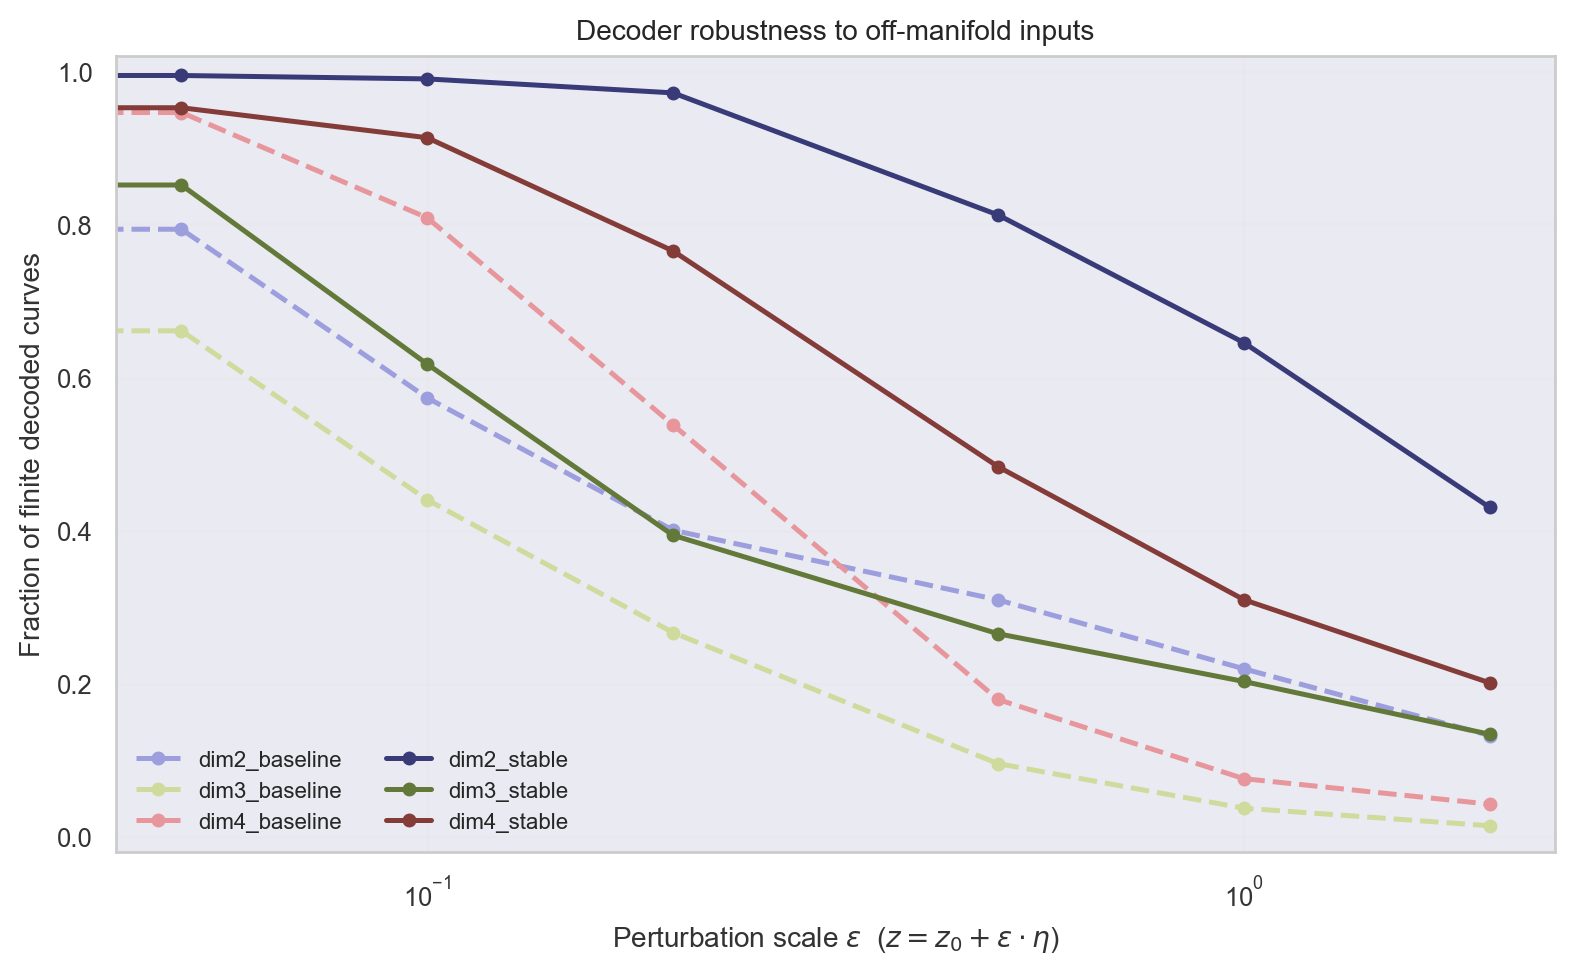
\includegraphics[width=0.85\textwidth]{Figures/Pricing/fig_decoder_robustness.png}
    \caption{Decoder finite-decoding fraction versus isotropic perturbation scale \(\varepsilon\).}
    \label{fig:decoder_robustness}
\end{figure}

\begin{table}[H]
\centering
\caption{Fraction of decoded discount curves that are fully finite, as a function of perturbation scale $\varepsilon$. Each cell averages over 200 EUR curves $\times$ 50 isotropic Gaussian draws $= 10{,}000$ test points. All decoders handle $\varepsilon = 0$ perfectly (on-manifold); robustness degrades sharply for displacements above $\varepsilon \approx 0.5$.}
\label{tab:decoder_robustness}
\small
\begin{tabular}{lrrrrrrr}
\toprule
Model & $\varepsilon = 0.0$ & $\varepsilon = 0.05$ & $\varepsilon = 0.1$ & $\varepsilon = 0.2$ & $\varepsilon = 0.5$ & $\varepsilon = 1.0$ & $\varepsilon = 2.0$ \\
\midrule
\texttt{dim2_baseline} & 1.000 & 0.794 & 0.574 & 0.401 & 0.310 & 0.220 & 0.132 \\
\texttt{dim3_baseline} & 1.000 & 0.661 & 0.440 & 0.267 & 0.096 & 0.038 & 0.015 \\
\texttt{dim4_baseline} & 1.000 & 0.946 & 0.809 & 0.538 & 0.180 & 0.076 & 0.043 \\
\texttt{dim2_stable} & 1.000 & 0.995 & 0.990 & 0.972 & 0.812 & 0.646 & 0.430 \\
\texttt{dim3_stable} & 1.000 & 0.852 & 0.618 & 0.394 & 0.265 & 0.203 & 0.134 \\
\texttt{dim4_stable} & 1.000 & 0.952 & 0.913 & 0.765 & 0.484 & 0.310 & 0.201 \\
\bottomrule
\end{tabular}
\end{table}

Figure~\ref{fig:decoder_robustness} and Table~\ref{tab:decoder_robustness} show that all decoders handle the unperturbed encoded states, corresponding to \(\varepsilon=0\). As the perturbation scale increases, the fraction of finite decoded curves declines. The stable decoders are more robust than the baseline decoders of the same dimension, but robustness still deteriorates for moderate perturbations. This suggests that reconstruction training gives the decoder a limited reliable operating region around the encoded data, rather than a guarantee of valid decoding throughout latent space.

\item[Where the SDE actually goes.]
The previous diagnostic shows how the decoder behaves under controlled perturbations. The next question is whether the simulated latent SDE reaches perturbation sizes where the decoder becomes unreliable. To test this, we simulate \(1{,}000\) paths to \(T_e=5\)Y and compute the terminal displacement
\[
\|z_{T_e}^{(m)}-z_0\|.
\]
This is the Euclidean distance in latent space between the initial encoded state \(z_0\) and the simulated state at option expiry on path \(m\). It measures how far the pricing simulation moves the latent state away from the starting curve.

\begin{figure}[H]
    \centering
    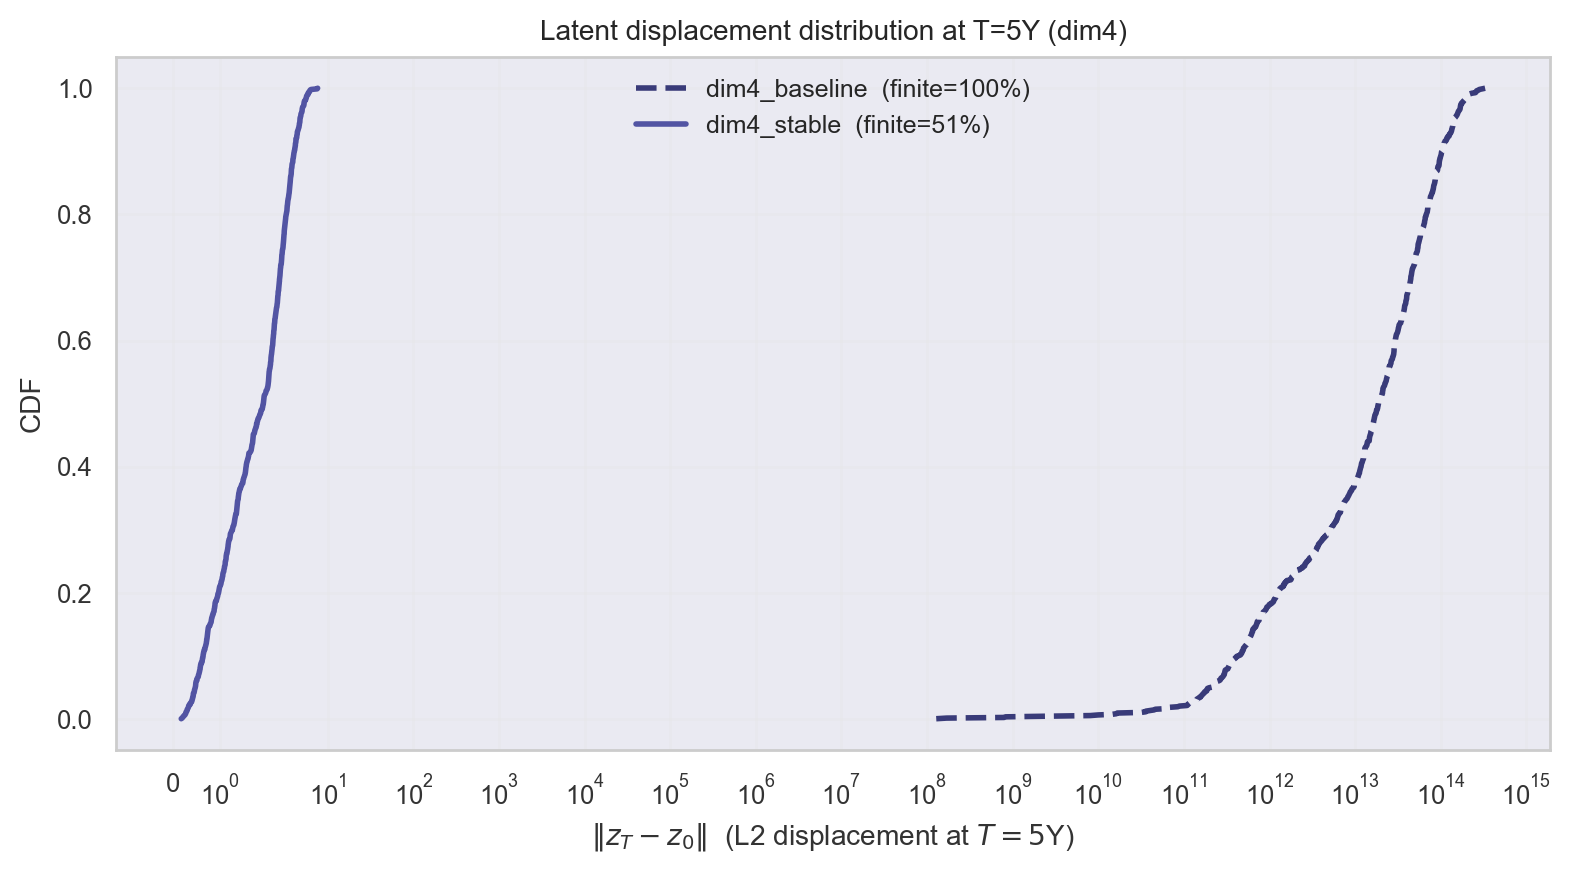
\includegraphics[width=0.85\textwidth]{Figures/Pricing/fig_latent_displacement_cdf.png}
    \caption{CDF of the terminal latent displacement \(\|z_{T_e}-z_0\|\) at \(T_e = 5\)Y for the dim4 baseline and stable models. The horizontal axis is shown on a symlog scale.}
    \label{fig:latent_displacement_cdf}
\end{figure}

\begin{table}[H]
\centering
\caption{Statistics of $\|z_T - z_0\|$ at $T_e = 5$Y under Euler--Maruyama simulation ($N=1000$ paths, $\Delta t = 1/12$ y) and the corresponding fraction of paths that decode to finite discount curves. The baseline SDE diverges by thirteen orders of magnitude; the stable SDE produces well-behaved displacements but the recon-only decoder cannot handle them.}
\label{tab:displacement_summary}
\small
\begin{tabular}{lrrrrr}
\toprule
Model & Mean & Median & p95 & Max & Finite \% \\
\midrule
\texttt{dim4\_baseline} & 3.87e+13 & 1.88e+13 & 1.44e+14 & 3.3e+14 & 100.0\% \\
\texttt{dim4\_stable} & 2.15 & 1.9 & 4.72 & 7.59 & 51.2\% \\
\bottomrule
\end{tabular}
\end{table}

Figure~\ref{fig:latent_displacement_cdf} plots the cumulative distribution function of the terminal displacement. For any value on the horizontal axis, the curve shows the fraction of Monte Carlo paths with terminal displacement below that value. The baseline distribution lies far to the right, indicating extremely large latent movements. The stable distribution is much more controlled and concentrated at moderate distances from \(z_0\).

This explains the different pricing failures. The baseline model sends the latent state far outside the region represented in the training data. Even if the decoder returns finite numerical outputs, these outputs are extreme extrapolations and should not be interpreted as reliable discount curves. The stable model avoids this explosive behaviour, which is the intended effect of the stability restriction. However, the stable paths still move far enough away from the encoded starting point that they enter the range where the decoder robustness test showed frequent failures. Hence the stable model is dynamically well behaved, but the decoder is not necessarily reliable on all latent states visited during pricing.

\item[Drift and diffusion contributions.]
To understand where the stable model's latent movement comes from, we decompose the
simulated motion into drift-only and diffusion-only contributions. This separates the roles
of the drift network \(\mathcal K\) and the diffusion network \(\mathcal H\).

\begin{table}[H]
\centering
\caption{Decomposition of the 5-year displacement into diffusion and drift components for dim4 models. The \emph{Diff. annualised} column reports the one-step diffusion-only displacement scaled by $\sqrt{N_{\rm steps}}$ (approximate cumulative diffusion contribution). The \emph{Drift only} column reports $\|z_T - z_0\|$ with $H=0$ over $T = 5$Y. Stable's drift is bounded by mean reversion; baseline's drift alone explodes to $\sim 8\times 10^3$.}
\label{tab:hk_decomposition}
\small
\begin{tabular}{lrrrrr}
\toprule
Model & $\|z_0 - z^*\|$ & $\bar{\sigma}_H$ & Diff. annualised & Drift only ($T=5$Y) & Full ($T=5$Y) \\
\midrule
\texttt{dim4\_baseline} & 0.178 & 0.967 & 3.956 & 8.37e+03 & 3.87e+13 \\
\texttt{dim4\_stable} & 9.527 & 1.054 & 4.613 & 0.14 & 2.15 \\
\bottomrule
\end{tabular}
\end{table}

The baseline model is included in Table~\ref{tab:hk_decomposition} as a reference. Its large displacement is mainly a consequence of the instability already discussed in the simulation chapter. In particular, the drift can generate explosive movement along unstable eigendirections.

The stable model behaves differently. The stability restriction ensures that the linear drift has only negative eigenvalues, so the drift-only trajectory remains bounded. The full simulated displacement is therefore mainly driven by the diffusion term, with the mean-reverting drift acting as a restoring force. Table~\ref{tab:hk_decomposition} shows that the drift-only five-year displacement is small, while the full displacement is much larger. Thus, for the stable model, the pricing-relevant movement away from \(z_0\) is primarily diffusion-driven.

\item[An apparent paradox in the stable variant.]
One might expect the stable drift to dominate the simulation because the stable equilibrium
\[
z^* = -M^{-1}N_{\mathcal K}
\]
lies far from a typical encoded EUR curve. In the dim4 stable model, \(\|z^*-z_0\|\) is approximately \(9.5\). At first sight, this suggests that the mean-reverting drift should pull the latent state strongly toward the equilibrium, producing a large drift-driven displacement over five years.

\begin{table}[H]
\centering
\caption{Eigenvector alignment of $(z^* - z_0)$ for dim4 stable. The slowest eigenvalue ($|\lambda| \approx 0.002$) absorbs essentially all of the misplacement. Over $T = 5$Y the slow direction barely activates ($1 - e^{\lambda T} \approx 0.008$), so the equilibrium misplacement contributes $\approx 0.14$ to the realised displacement, despite $\|z^* - z_0\| \approx 9.5$.}
\label{tab:eigenvector_alignment}
\small
\begin{tabular}{rrrrrr}
\toprule
Mode & $\lambda$ & timescale (y) & $|a_i|$ & $|1-e^{\lambda T}|$ & contribution \\
\midrule
0 & -5.0763 & 0.2 & 0.068 & 1.0000 & 0.0675 \\
1 & -2.3136 & 0.4 & 0.021 & 1.0000 & 0.0208 \\
2 & -1.0441 & 1.0 & 0.093 & 0.9946 & 0.0921 \\
3 & -0.0016 & 610.5 & 9.526 & 0.0082 & 0.0777 \\
\bottomrule
\end{tabular}
\end{table}

Table~\ref{tab:eigenvector_alignment} explains why this does not happen. The vector \(z^*-z_0\) is almost entirely aligned with the slowest eigenvector of \(\mathcal K\). The corresponding eigenvalue is very close to zero, giving a mean-reversion timescale of roughly 600 years. Over a five-year pricing horizon, this direction barely moves. Hence the large distance between \(z_0\) and \(z^*\) is structurally present, but dynamically almost inactive at swaption-pricing horizons. The realised drift-only displacement is therefore small, despite the equilibrium being far away.

\end{description}

The diagnostics identify a first barrier: decoder coverage is incomplete for simulated latent states. A diffusion scale \(s^*\) per expiry can reduce the magnitude of simulated paths (calibrated values: \(s^*(1\mathrm{Y})=0.129\), \(s^*(5\mathrm{Y})=0.133\), \(s^*(10\mathrm{Y})=0.141\)), which lowers the vol level from roughly six times market to within \(72\) bp. However, a second and more fundamental problem remains. We turn to that now.

%----------------------------------------------------------
\subsection{The Forward Bias: Historical vs Risk-Neutral Drift}
\label{sec:pricing_diagnostics}
%----------------------------------------------------------

After controlling the diffusion level, the residual pricing error has a systematic structure: the model-implied distribution of the forward swap rate at expiry is centred below the market forward. This is not a volatility-scale problem but a drift problem.

The Bachelier Delta identity provides a convenient benchmark. In the Bachelier model, the payer Delta is
\[
\Delta
=
\mathcal N\mathcal A_0\Phi(d),
\qquad
d=
\frac{F-K}{\sigma_N\sqrt{T_e}}.
\]
For a correctly centred at-the-money swaption, \(F=K=F_0\), so \(d=0\). The corresponding exercise probability is therefore
\[
\Phi(0)=50\%.
\]
Equivalently, under the annuity measure, the forward swap rate should satisfy the martingale condition
\[
\mathbb E^{\mathbb Q^{\mathcal A}}[S_{T_e}] = F_0.
\]
If the simulated distribution of \(S_{T_e}\) is not centred at \(F_0\), then the market at-the-money strike \(K=F_0\) is no longer at the money from the model's perspective.

This forward bias is estimated from payer--receiver parity. For payer and receiver prices computed at the same strike \(K=F_0\), the model-implied forward is
\[
F_{\mathrm{mod}}
=
F_0
+
\frac{
V_{\mathrm{pay}}-V_{\mathrm{rec}}
}{
\mathcal N\mathcal A_0
},
\]
so the forward bias is
\begin{equation}
  \text{forward bias}
  =
  F_{\mathrm{mod}}-F_0
  =
  \frac{
  V_{\mathrm{pay}}-V_{\mathrm{rec}}
  }{
  \mathcal N\mathcal A_0
  }.
  \label{eq:forward_bias}
\end{equation}
A negative value means that the model-implied distribution is centred below the market forward rate. We standardise the bias by the straddle-implied volatility
\[
  \sigma_{\mathrm{str}}
  =
  \frac{V_{\mathrm{pay}} + V_{\mathrm{rec}}}{2}
  \cdot
  \frac{\sqrt{2\pi}}{\mathcal N\mathcal A_0\sqrt{T_e}},
\]
which measures the width of the model's distribution around the strike without directional assumption. This gives the effective exercise probability
\begin{equation}
  d_{\mathrm{eff}}
  =
  \frac{\text{forward bias}}{\sigma_{\mathrm{str}}\sqrt{T_e}},
  \qquad
  p_{\mathrm{eff}}
  =
  \Phi(d_{\mathrm{eff}}).
  \label{eq:p_eff}
\end{equation}
Under a correctly centred model, \(d_{\mathrm{eff}}=0\) and \(p_{\mathrm{eff}}=50\%\). Deviations from \(50\%\) quantify how far the model's swap-rate distribution is shifted relative to the market forward.

\paragraph{Results.}
Table~\ref{tab:delta_diagnostic} reports the per-cell forward bias and effective exercise probability across the nine expiry--tenor cells. Two findings stand out.

First, the forward bias is consistently negative across all nine cells, ranging from \(-18\) bp for the \(10\mathrm{Y}{\times}1\mathrm{Y}\) cell to \(-694\) bp for the \(1\mathrm{Y}{\times}5\mathrm{Y}\) cell. The model-implied distribution of \(S_{T_e}\) is therefore systematically below \(F_0\) across the expiry--tenor grid. This is consistent with the drift \(\mathcal K\) having been estimated from historical yield-curve dynamics rather than from the risk-neutral martingale condition required for pricing.

Second, the effective exercise probabilities range from \(24\%\) for the \(1\mathrm{Y}{\times}5\mathrm{Y}\) cell to \(49\%\) for the \(10\mathrm{Y}{\times}1\mathrm{Y}\) cell, with an overall average of approximately \(35\%\). The short-expiry cells are furthest from the \(50\%\) benchmark, consistent with the rate level having the greatest impact on shorter horizons.

\begin{table}[H]
\centering
\caption{Per-cell forward bias and effective ATM exercise probability at the expiry-level calibrated scale. The forward bias $\mathbb{E}^{\mathbb{Q}_\mathcal{A}}[S_T] - F_0$ is measured directly from put-call parity: $(V_{\mathrm{pay}} - V_{\mathrm{rec}})/\mathcal{A}_0$. The effective exercise probability $p_{\mathrm{eff}} = \Phi(d_{\mathrm{eff}})$ where $d_{\mathrm{eff}} = \text{forward bias} / (\sigma_{\mathrm{str}}\sqrt{T_e})$ measures how far the model's $\mathbb{Q}$ distribution is shifted relative to its own width. Under a correctly specified risk-neutral model: forward bias $= 0$ and $p_{\mathrm{eff}} = 50\%$. Deviations quantify the failure of $\mathcal{K}$ to satisfy the annuity-measure martingale condition.}
\label{tab:delta_diagnostic}
\begin{tabular}{@{}ccrrrrr@{}}
\toprule
\textbf{Exp} & \textbf{Ten} & $\sigma_{\mathrm{mkt}}$ \textbf{(bp)} & $\sigma_{\mathrm{str}}$ \textbf{(bp)} & \textbf{Fwd bias (bp)} & $d_{\mathrm{eff}}$ & $p_{\mathrm{eff}}$ \textbf{(\%)} \\
\midrule
1 & 1 & 60 & 588 & $-255$ & $-0.43$ & 33.3 \\
1 & 5 & 73 & 991 & $-694$ & $-0.70$ & 24.2 \\
1 & 10 & 90 & 384 & $-207$ & $-0.53$ & 29.8 \\
\addlinespace[2pt]
5 & 1 & 56 & 226 & $-85$ & $-0.16$ & 43.8 \\
5 & 5 & 58 & 494 & $-665$ & $-0.60$ & 27.4 \\
5 & 10 & 53 & 205 & $-167$ & $-0.36$ & 36.2 \\
\addlinespace[2pt]
10 & 1 & 48 & 143 & $-18$ & $-0.03$ & 48.8 \\
10 & 5 & 45 & 336 & $-587$ & $-0.55$ & 29.1 \\
10 & 10 & 43 & 148 & $-145$ & $-0.30$ & 38.2 \\
\midrule
\textbf{Overall} & & 58 & 376 & $-313$ & & 34.6 \\
\bottomrule
\end{tabular}
\end{table}

\begin{figure}[H]
  \centering
  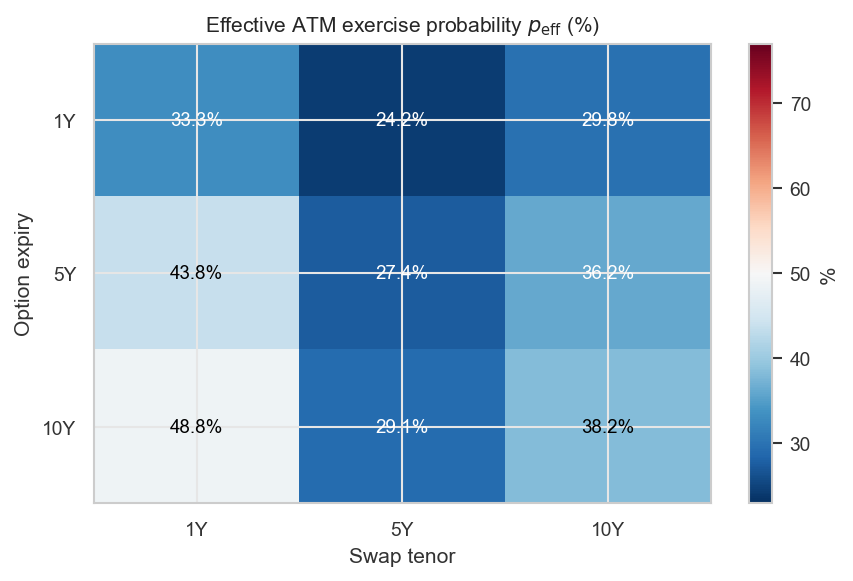
\includegraphics[width=0.72\textwidth]{Figures/TrainingResults/dim4_stable_hscale/delta_diagnostic/fig_exercise_prob.png}
  \caption{Effective ATM exercise probability \(p_{\mathrm{eff}}\) per cell at the expiry-level calibrated scale. The Bachelier benchmark is \(50\%\). All cells are below \(50\%\), indicating a systematic downward bias in the model-implied swap-rate distribution.}
  \label{fig:exercise_prob}
\end{figure}

A scalar diffusion scale can adjust the spread of the simulated distribution, but it cannot recenter the distribution around \(F_0\). The source of the remaining error is structural: the drift \(\mathcal K\) simultaneously acts as the historical drift recovered from encoded yield-curve dynamics and as the risk-neutral drift governing the pricing simulation. These two roles make conflicting demands. The next section addresses this by introducing a separate risk-neutral drift parameterised through the Girsanov market price of risk.


%=========================================================
\section{The Lambda Market Price of Risk}
\label{sec:lyashenko}
%=========================================================

The forward-bias diagnostic in the previous section points to a structural mismatch: the historical drift \(\mathcal K\) is not the risk-neutral drift required for swaption pricing. The direct approach of training a separate unrestricted \(\mathcal K^{\mathbb Q}\) against swaption prices was tested but failed: although the pricing loss decreased, \(\mathcal H\) needed to move for vol calibration, and \(\mathcal H\) enters the bond-pricing ODE through the diffusion covariance \(\Sigma(z)=\mathcal H(z)\mathcal H(z)^\top\). The result was that reconstruction RMSE degraded from \(5.3\) bp to \(66\) bp and the fraction of finite pricing paths fell from \(52\%\) to \(32\%\). Any parameter that appears inside the no-arbitrage ODE cannot be trained against a pricing objective without corrupting reconstruction.

Girsanov's theorem provides a structured alternative that avoids this problem.

\subsection{Girsanov Structure}
\label{subsec:lyashenko_girsanov}

Let \(W^{\mathbb P}\) be a Brownian motion under the historical measure and let
\(\lambda_t\) denote the market price of risk. Under the change of measure,
\[
    W^{\mathbb Q}_t
    =
    W^{\mathbb P}_t
    +
    \int_0^t \lambda_s\,ds
\]
is a Brownian motion under the risk-neutral measure. If the latent dynamics under
\(\mathbb P\) are
\begin{equation}
    dz_t
    =
    \mathcal K^{\mathbb P}(z_t)\,dt
    +
    \mathcal H(z_t)\,dW^{\mathbb P}_t,
    \label{eq:P_sde}
\end{equation}
then the corresponding \(\mathbb Q\)-measure dynamics are
\begin{equation}
    dz_t
    =
    \Bigl[
        \mathcal K^{\mathbb P}(z_t)
        -
        \mathcal H(z_t)\lambda(z_t)
    \Bigr]dt
    +
    \mathcal H(z_t)\,dW^{\mathbb Q}_t.
    \label{eq:Q_sde}
\end{equation}
Hence the risk-neutral drift is
\[
    \mathcal K^{\mathbb Q}(z)
    =
    \mathcal K^{\mathbb P}(z)
    -
    \mathcal H(z)\lambda(z).
\]
With the affine specification \(\lambda(z)=\Lambda z\), this becomes
\[
    \mathcal K^{\mathbb Q}(z)
    =
    \mathcal K^{\mathbb P}(z)
    -
    \mathcal H(z)\Lambda z.
\]
The learnable object is then the matrix \(\Lambda\). Crucially, \(\Lambda\) appears only in the simulation and the pricing ODE. It does not appear in the reconstruction ODE, which continues to use \(\mathcal K^{\mathbb P}\). Reconstruction is therefore completely insulated from training. With \(\ell_2\) regularisation on \(\Lambda\), the risk-neutral correction is kept proportional to the diffusion directions of \(\mathcal H\), bounding the shift in the risk-neutral equilibrium \(z^*_{\mathbb Q}\) and keeping pricing paths near the decoder's operating region. This is closely related to the framework of \citet{Lyashenko2019}, where the separation between historical and risk-neutral term-structure dynamics is imposed at the model-design level.

\subsection{Implementation}
\label{subsec:lambda_implementation}

The separation is implemented through a \texttt{LambdaMPR} module:
\[
    \mathcal K^{\mathbb Q}(z)
    =
    \mathcal K^{\mathbb P}(z)
    -
    L(z)\,\Lambda\, z,
\]
where \(L(z)\) is the Cholesky factor of \(\mathcal H(z)\mathcal H(z)^\top\), computed from the frozen \(\mathcal H\) with no gradient flow. All original network weights \(\mathcal K^{\mathbb P}\), \(\mathcal H\), and \(\mathcal G\) remain frozen. The simulation and pricing ODE use \(\mathcal K^{\mathbb Q}\) while reconstruction uses \(\mathcal K^{\mathbb P}\). For the four-dimensional stable model, \(\Lambda\) is a \(4\times4\) matrix initialised at zero, giving \(16\) trainable parameters and ensuring training starts with \(\mathcal K^{\mathbb Q}=\mathcal K^{\mathbb P}\).

The diffusion level is controlled by the expiry-level scales calibrated from the vol level prior to Lambda training: \(s^*(1\mathrm{Y})=0.129\), \(s^*(5\mathrm{Y})=0.133\), \(s^*(10\mathrm{Y})=0.141\). These are applied as a multiplicative scaling of the simulation noise at each time step and do not modify any network weights.

The training objective is
\[
    \mathcal{L}
    =
    \mathcal{L}_{\mathrm{price}}
    +
    \lambda_{\mathrm{eig}}\,\mathcal{L}_{\mathrm{eig}}
    +
    \lambda_{\ell_2}\,\|\Lambda\|_F^2,
\]
where \(\mathcal{L}_{\mathrm{price}}\) is the mean-squared normal-volatility error across a random subsample of swaption quotes at each step, \(\mathcal{L}_{\mathrm{eig}}\) penalises positive real parts of the eigenvalues of the linearised \(\mathcal K^{\mathbb Q}\) to maintain mean reversion under \(\mathbb Q\), and the \(\ell_2\) term bounds \(\Lambda\) relative to \(\mathcal K^{\mathbb P}\). The model is trained for \(1{,}000\) epochs with Adam.

\subsection{Results}
\label{subsec:lambda_results}

Table~\ref{tab:lambda_training_progress} reports key metrics at selected checkpoints.

\begin{table}[H]
\centering
\caption{Training progress for the \(\Lambda\)-MPR run. Reconstruction RMSE is evaluated
using the frozen \(\mathcal K^{\mathbb P}\) and the frozen \(\mathcal H\). Path finite fraction
is the share of \(N_{\mathrm{MC}}=256\) paths producing finite decoded bond curves.
\(\|\Lambda\|_F\) is the Frobenius norm of the learned \(4\times4\) matrix.}
\label{tab:lambda_training_progress}
\small
\begin{tabular}{@{}rrrrrr@{}}
\toprule
\textbf{Epoch} & \textbf{Pricing loss} & \textbf{Path finite} & \textbf{Recon RMSE (bp)} & \(\boldsymbol{\lambda_{\min}(\mathcal K^{\mathbb Q})}\) & \(\boldsymbol{\|\Lambda\|_F}\) \\
\midrule
    0 & 1.359 & 78\% & 5.30 & 0.0016 & 0.000 \\
  200 & 0.186 & 73\% & 5.30 & 0.167  & 0.269 \\
  400 & 0.066 & 76\% & 5.30 & 0.282  & 0.412 \\
  600 & 0.203 & 80\% & 5.30 & 0.316  & 0.455 \\
  800 & 1.318 & 80\% & 5.30 & 0.322  & 0.465 \\
  999 & 0.046 & 74\% & 5.30 & 0.324  & 0.467 \\
\bottomrule
\end{tabular}
\end{table}

The reconstruction RMSE is constant at \(5.30\) bp throughout the entire run. Because both \(\mathcal H\) and \(\mathcal K^{\mathbb P}\) are frozen, the no-arbitrage ODE coefficients and the decoded bond prices are completely unaffected by training. Reconstruction is structurally protected.

The path finite fraction remains in the range \(73\)--\(80\%\) throughout, compared with the fall from \(52\%\) to \(32\%\) in the unconstrained experiment. The \(\ell_2\) regularisation on \(\Lambda\) bounds the size of the Girsanov correction, limiting how far the risk-neutral equilibrium shifts from \(z^*_{\mathbb P}\) and keeping pricing paths within the decoder's operating region.

The Frobenius norm \(\|\Lambda\|_F\) stabilises near \(0.467\) from around epoch \(600\), and the smallest eigenvalue of \(\mathcal K^{\mathbb Q}\) plateaus at \(0.324\). In mean-reversion terms, the slowest latent direction changes from approximately \(1{,}570\) years under \(\mathbb P\) (eigenvalue \(6.4\times10^{-4}\)) to roughly \(3.1\) years under \(\mathbb Q\) (eigenvalue \(0.324\)). This is the dominant Girsanov correction.

\paragraph{Structure of the learned \(\Lambda\).}
The final checkpoint yields
\[
\Lambda
=
\begin{pmatrix}
 0.242 & -0.198 &  0.119 & -0.211 \\
-0.016 & -0.023 &  0.068 & -0.041 \\
 0.051 &  0.018 & -0.079 &  0.068 \\
 0.153 & -0.109 &  0.014 & -0.077
\end{pmatrix}.
\]
The row norms are \(\|{\Lambda}_{0,\cdot}\|=0.395\), \(\|{\Lambda}_{1,\cdot}\|=0.084\), \(\|{\Lambda}_{2,\cdot}\|=0.117\), \(\|{\Lambda}_{3,\cdot}\|=0.203\). The first row dominates by a factor of roughly two over the next largest. This first row corresponds to the near-unit-root latent direction. The correction \(\mathcal H(z)\Lambda z\) is therefore concentrated in the direction of the level factor, increasing its mean-reversion speed under the pricing measure. Duration risk---the sensitivity of a fixed-income portfolio to parallel shifts in the yield curve---is widely documented as the dominant source of the term premium in government bond markets. The \(\Lambda\)-MPR training identifies the same direction automatically.

\paragraph{Per-cell vol errors.}
Table~\ref{tab:lambda_per_cell_final} and Figure~\ref{fig:vol_surface} report the per-cell ATM vol errors on the EUR test set. Figure~\ref{fig:vol_error_timeseries} shows how the vol error evolves over the historical test period for each cell.

\begin{table}[H]
\centering
\caption{Per-cell ATM vol errors at the final $\Lambda$-MPR checkpoint (ep\,999, EUR test set). Model implied vol is the payer-derived ATM normal vol (basis points). Forward bias $= (V_{\mathrm{pay}} - V_{\mathrm{rec}})/\mathcal{A}_0 \times 10{,}000$\,bp; the risk-neutral benchmark is $0$.}
\label{tab:lambda_per_cell_final}
\small
\begin{tabular}{@{}ccrrrrr@{}}
\toprule
\textbf{Exp} & \textbf{Ten} & \textbf{Mkt vol (bp)} & \textbf{Mod vol (bp)} & \textbf{MAE (bp)} & \textbf{RMSE (bp)} & \textbf{Fwd bias (bp)} \\
\midrule
  1Y & 1Y & 56 & 79 & 28.4 & 39.9 & -501.3 \\
  1Y & 5Y & 55 & 15 & 39.7 & 42.1 & -772.3 \\
  1Y & 10Y & 191 & 64 & 126.4 & 221.0 & -261.4 \\
  \midrule
  5Y & 1Y & 47 & 20 & 26.8 & 28.0 & -488.4 \\
  5Y & 5Y & 102 & 27 & 74.3 & 101.2 & -996.9 \\
  5Y & 10Y & 92 & 36 & 56.2 & 82.1 & -343.2 \\
  \midrule
  10Y & 1Y & 79 & 29 & 49.6 & 65.5 & -325.4 \\
  10Y & 5Y & 75 & 22 & 53.1 & 69.2 & -1060.9 \\
  10Y & 10Y & 69 & 22 & 49.2 & 63.0 & -389.9 \\
\bottomrule
\end{tabular}
\end{table}

\begin{figure}[H]
  \centering
  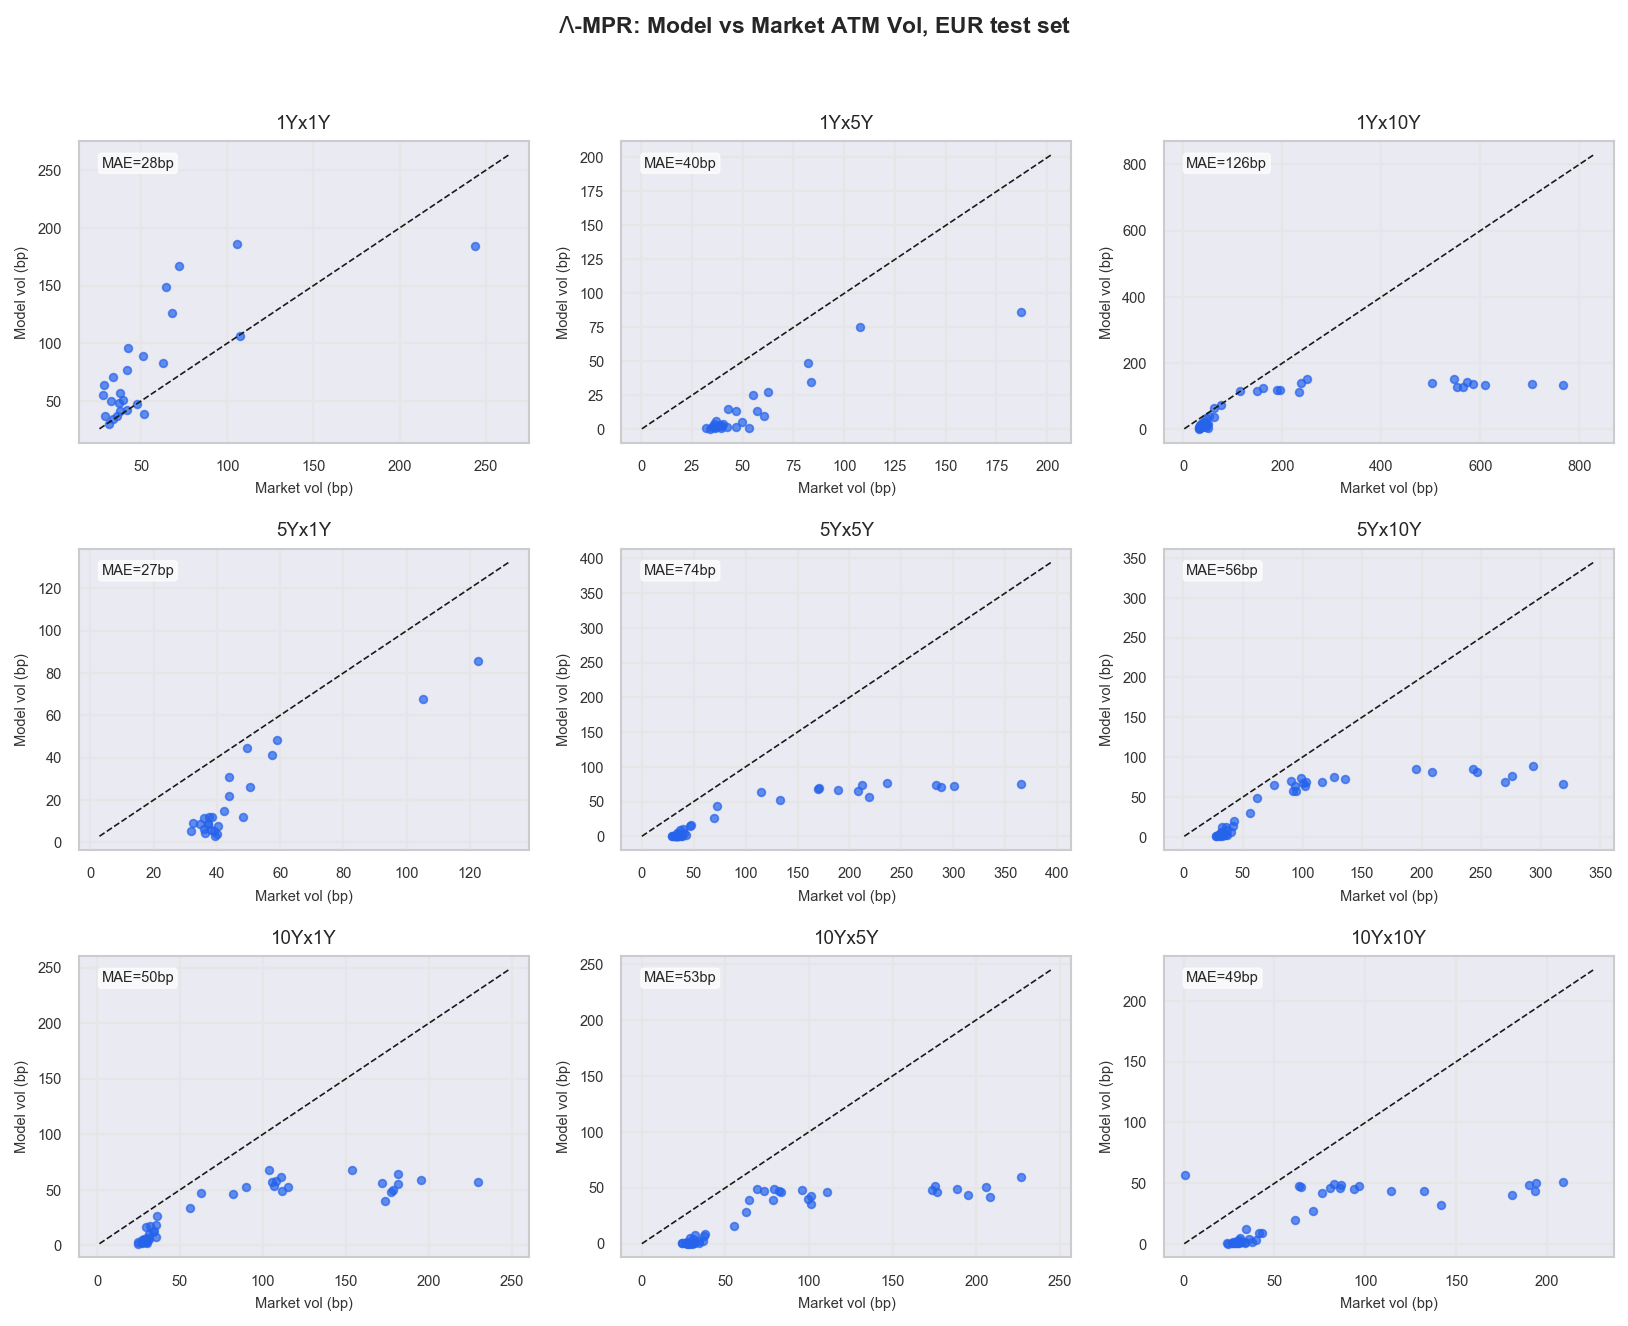
\includegraphics[width=\textwidth]{Figures/TrainingResults/dim4_stable_lambda_mpr/ep1000/eval/fig_vol_surface.png}
  \caption{Model vs market ATM implied vol (basis points) per expiry--tenor cell, EUR test set, \(\Lambda\)-MPR at epoch \(999\). Each dot is one observation date. The dashed line is the \(45^\circ\) reference.}
  \label{fig:vol_surface}
\end{figure}

\begin{figure}[H]
  \centering
  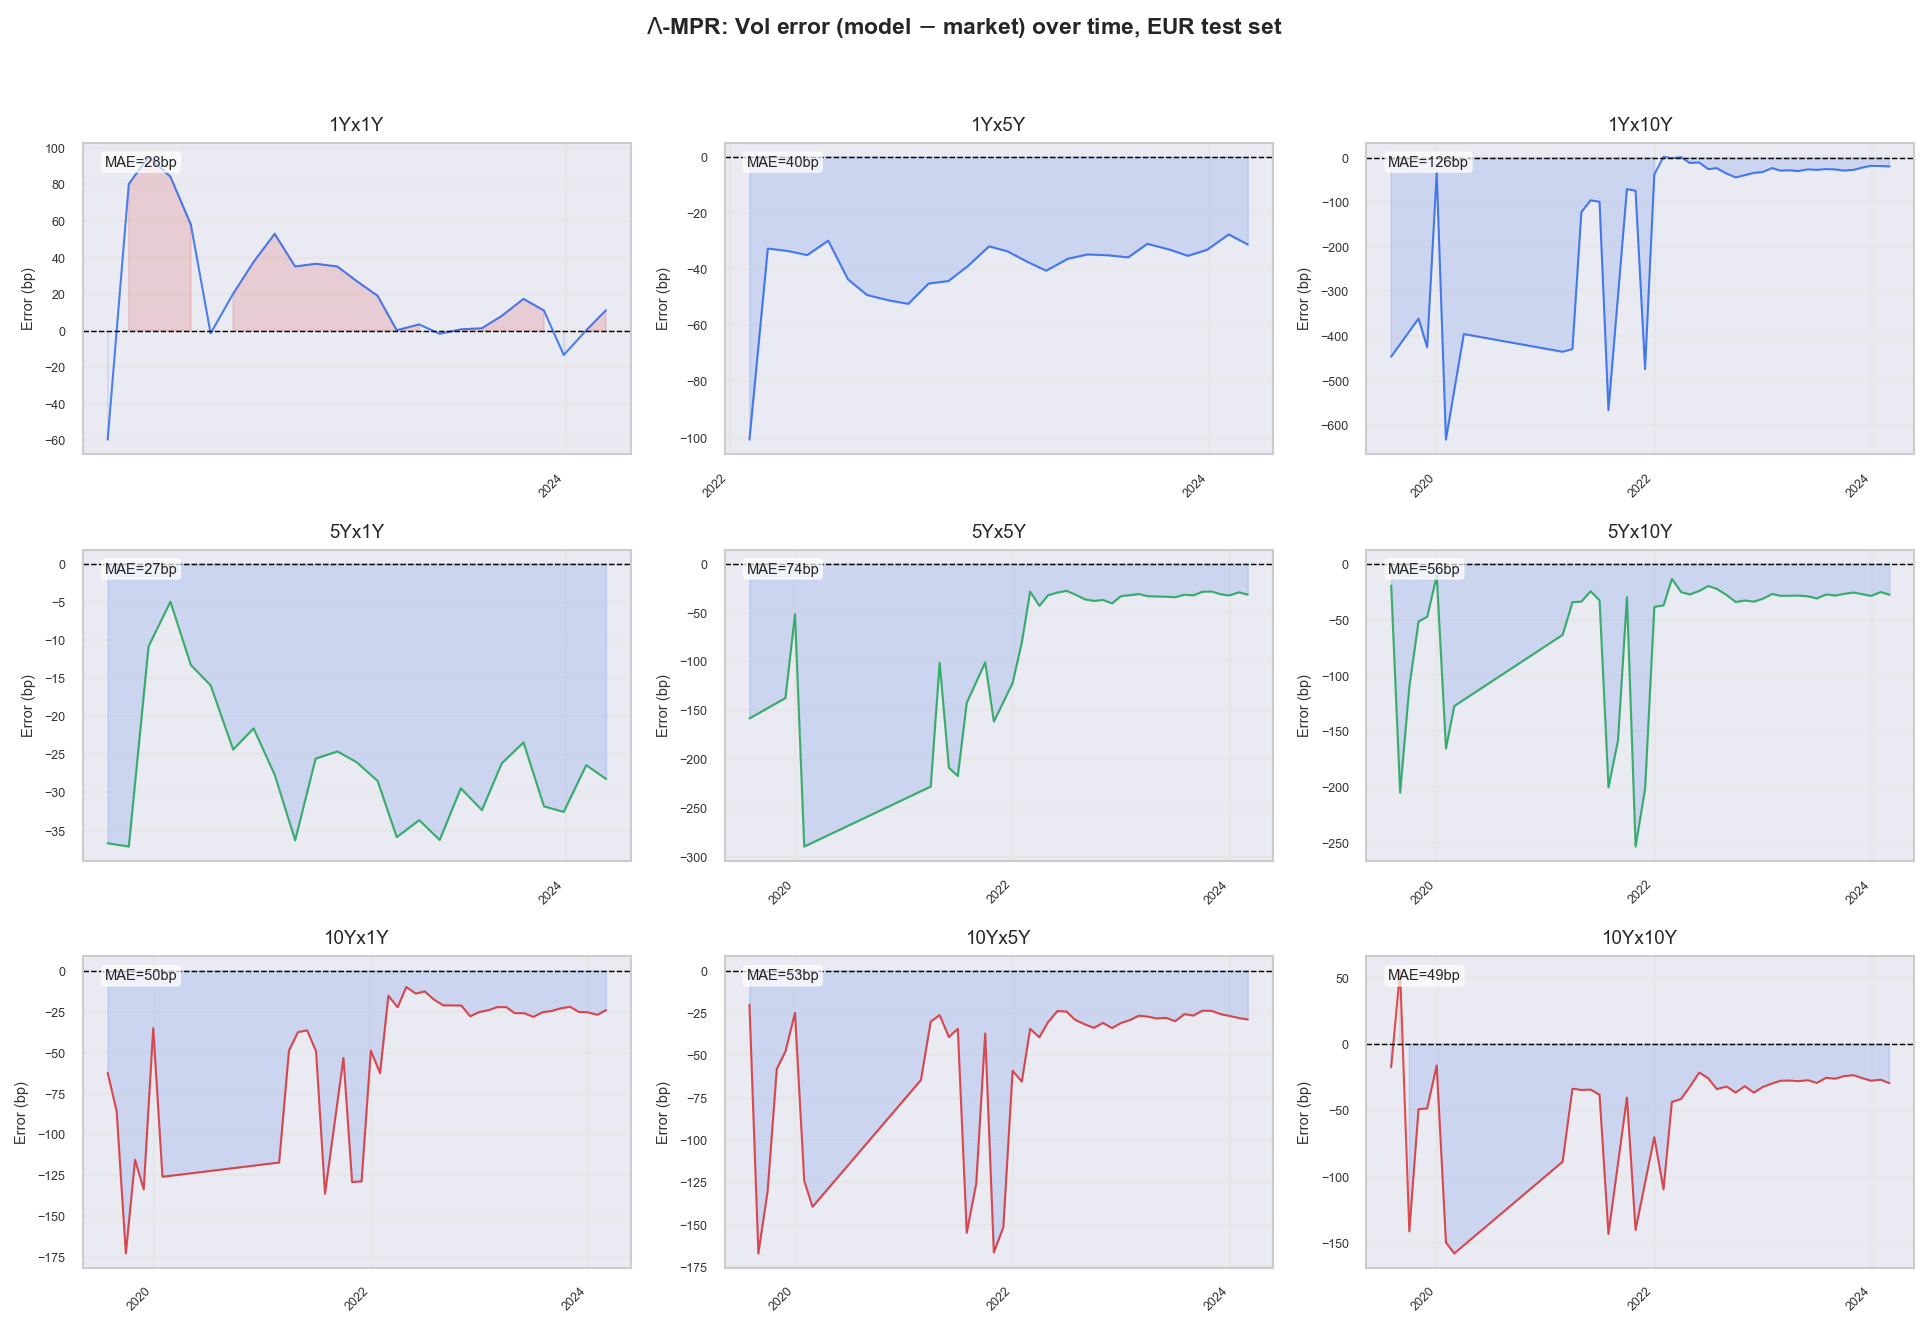
\includegraphics[width=\textwidth]{Figures/TrainingResults/dim4_stable_lambda_mpr/ep1000/eval/fig_vol_error_timeseries.png}
  \caption{Vol error (model\,$-$\,market, basis points) over calendar time per expiry--tenor cell, EUR test set. The dashed line is zero (perfect pricing). Red shading indicates over-pricing; blue shading indicates under-pricing.}
  \label{fig:vol_error_timeseries}
\end{figure}

\paragraph{Forward bias over time.}

\begin{figure}[H]
  \centering
  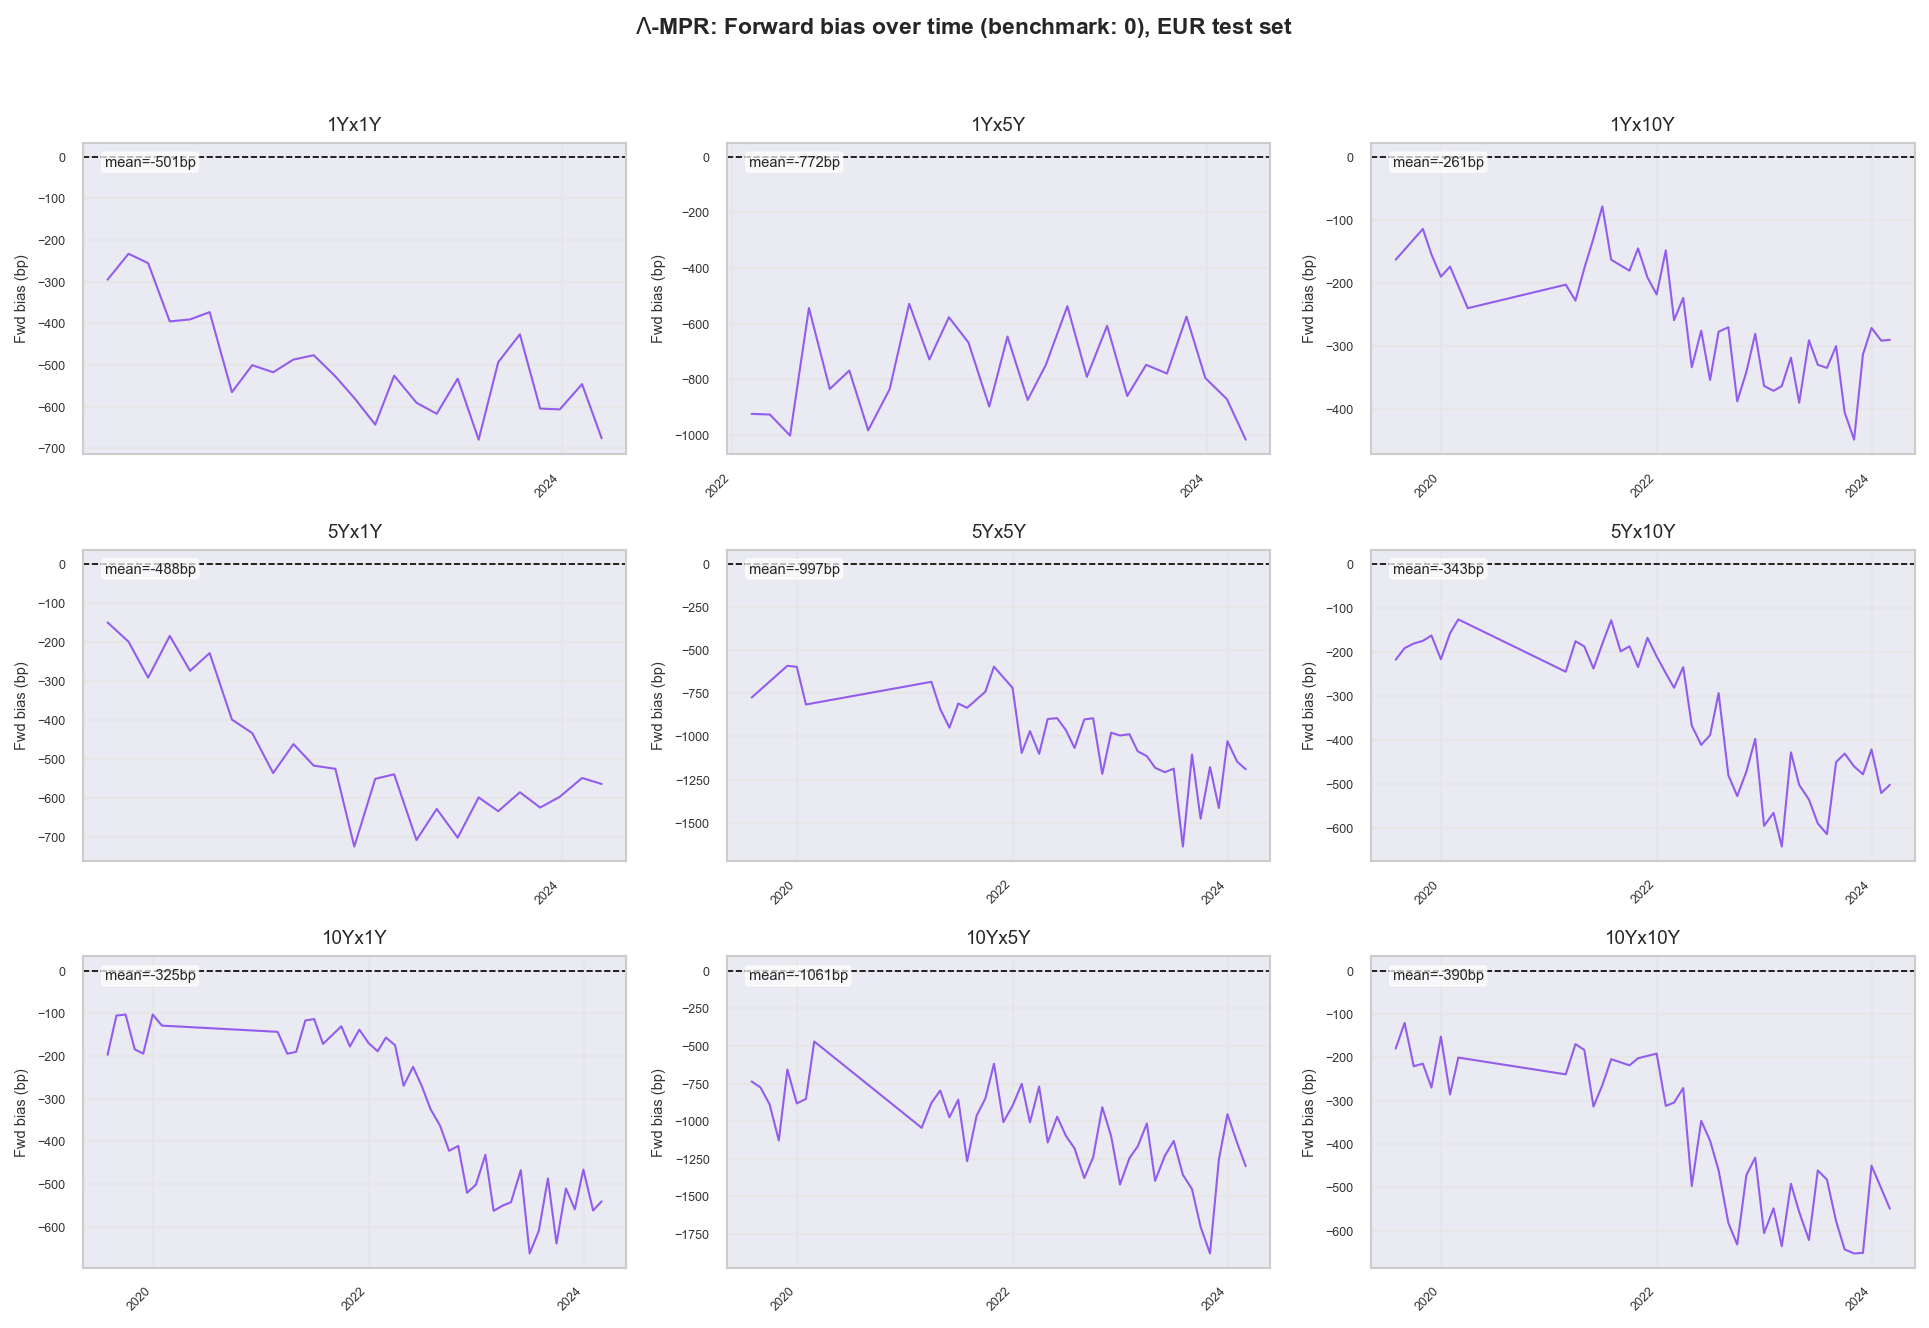
\includegraphics[width=\textwidth]{Figures/TrainingResults/dim4_stable_lambda_mpr/ep1000/eval/fig_forward_bias_timeseries.png}
  \caption{Residual forward bias (basis points) over calendar time per cell, EUR test set. The dashed line is zero (risk-neutral benchmark). Persistent deviations indicate dates where the Girsanov correction does not fully centre the swap-rate distribution.}
  \label{fig:forward_bias_timeseries}
\end{figure}

\paragraph{ATM volatility surface.}
The nine cells in the figures above form the ATM swaption volatility surface (vol cube) for the expiries \(1\)Y, \(5\)Y, \(10\)Y and tenors \(1\)Y, \(5\)Y, \(10\)Y. The scatter plots in Figure~\ref{fig:vol_surface} show the model's ability to reproduce the level and cross-sectional shape of market ATM vols. The per-cell MAE reported in Table~\ref{tab:lambda_per_cell_final} reflects the residual error after the Girsanov correction. The focus here is exclusively on ATM prices; extending to the full per-strike vol smile---where implied vol is plotted as a function of strike at each maturity---would require pricing payer and receiver swaptions at multiple strikes and is beyond the scope of this chapter.
